\newpage
\chapter{Transformation de mod{\`e}les}

En fonction des besoins et des projets, les moyens de sp{\'e}cifier les mod{\`e}les sont diff{\'e}rents. Il en est de m{\^e}me pour la transformation de mod{\`e}les.

\section{Transformation endog{\`e}ne}
Une transformation endog{\`e}ne (ou raffinement) de mod{\`e}le consiste {\`a} modifier le contenu d'un mod{\`e}le sans en changer le but ou la s{\'e}mantique. Il s'agit de rajouter des d{\'e}tails {\`a} un mod{\`e}le ou bien de le restructurer pour en am{\'e}liorer la conception. Par principe, le raffinement implique que les deux mod{\`e}les, le mod{\`e}le source et le mod{\`e}le cible, soient du m{\^e}me type, c'est-{\`a}-dire conformes au m{\^e}me m{\'e}ta-mod{\`e}le.

\noindent La figure~\ref{raffinement} ci-dessous repr{\'e}sente ce concept.

\begin{figure}[!ht]
	\centering
	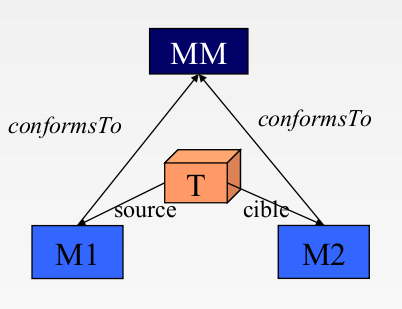
\includegraphics[scale=0.8]{endogene.png}
	\caption{Sch{\'e}ma d'une transformation par endog{\`e}ne (ou par raffinement)}
	\label{raffinement}

\end{figure}

\section{Transformation exog{\`e}ne}
Il s'agit d'une transformation entre deux espaces technologiques diff{\'e}rents. Les mod{\`e}les source et cible sont conformes {\`a} des m{\'e}ta-mod{\`e}les diff{\'e}rents. Par exemple la convertion d'un fichier XML en un sch{\'e}ma BDD.

\noindent La figure~\ref{projection} ci-dessous repr{\'e}sente ce concept.

\begin{figure}[!ht]
	\centering
	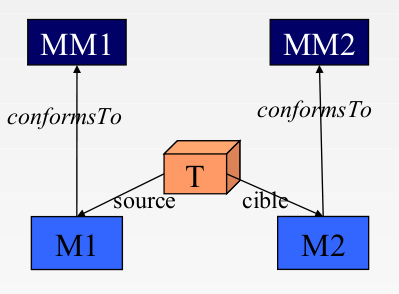
\includegraphics[scale=0.8]{exogene.png}
	\caption{Sch{\'e}ma d'une transformation exog{\`e}ne (ou par projection)}
	\label{projection}

\end{figure}

\section{Query}
La transformation de mod{\`e}le query est un type de transformation qui permet la transformation d'un m{\'e}ta-mod{\`e}le en texte (documentation ou code source).\\
Par exemple :
\begin{itemize}
\item transformer un mod{\`e}le UML vers du code Java;
\item contr{\^o}ler la coh{\'e}rence d'un mod{\`e}le UML en ecrivant une transformation qui affiche un diagnostic.
\end{itemize}

\section{Transformation g{\'e}n{\'e}riques}
Ce type de transformation se base sur les m{\'e}ta-m{\'e}tamod{\`e}les (mod{\`e}le MOF\protect\footnote{Meta-Object Facility}) et produit un mod{\`e}le cible g{\'e}n{\'e}rique, qui peut {\^e}tre r{\'e}utilisable. Elle peut {\^e}tre exog{\`e}ne ou endog{\`e}ne.
